\documentclass{beamer}
\usepackage[english]{babel}

\usepackage{amsmath,amssymb}
\usepackage{graphicx}
\usepackage{enumerate}
\usepackage[utf8]{inputenc} 
\usepackage[T1]{fontenc} 
\usepackage[english]{babel} 
% More space between lines in align
%\setlength{\mathindent}{0pt}

% Beamer theme
%\usetheme{ZMBZFMK}
\usefonttheme[onlysmall]{structurebold}
\mode<presentation>
\setbeamercovered{transparent=10}

% align spacing
\setlength{\jot}{0pt}

%\setbeamertemplate{navigation symbols}{}%remove navigation symbols

\title{Graphical models}
\author{Mateusz Małowiecki}
\institute[Instytut Informatyki Uniwersytetu Wrocławskiego]{}
\date{\today}
\DeclareUnicodeCharacter{2212}{-}
\begin{document}
\begin{frame}
  \titlepage
\end{frame}
\begin{frame}
  \frametitle{Reminder: Graphs}
    \begin{itemize}
      \item Consists of vertices and edges
      \item Vertices are adjacent if there is an edge between them
      %Vertices are adjacent if there is an edge between them​
      \item Path - sequence of vertices $x_1, x_2, ..., x_n$, such that $x_i$ and $x_{i+1}$ are adjacent 
      %Path – sequence of vertices x1, x2, xn; that xi and xi+1 are adjacent​
      \item Complete graph - graph in which all pairs of different vertices are adjacent 
      %Complete graph – graph in which all pairs of different vertices are adjacent​
      \item $H$ is subgraph of G iff $V(H) \subseteq V(G)$ and $E(H) \subseteq E(G)$  
      %H is subgraph of G iff V(H) is subset of V(G) and E(H) is subset of E(G)​
      \item Sparse graphs - graphs with relatively small number of edges
      %Sparse graphs – graphs with relatively small number of edges​
    \end{itemize}
\end{frame}
\begin{frame}
  \frametitle{Graphs - convention}
  \begin{itemize}
      \item Vertices represent random variables
      \item Edges mean random variables depedency
      \item We will talk only about directed graphs
      \item Edges in graph are parametrized by value
  \end{itemize}
\end{frame}
\begin{frame}
\frametitle{Challenges}
  \begin{itemize}
      \item Model selection
      \item Estimation of the edge parameters from data
      \item Computation of marginal vertex probabilities and exceptations, from their jonit distribution
  \end{itemize}
\end{frame}
\begin{frame}
\frametitle{Challenges}
  \begin{itemize}
      \item Model selection
      \item Estimation of the edge parameters from data
      \item Computation of marginal vertex probabilities and exceptations, from their jonit distribution
  \end{itemize}
\end{frame}
\begin{frame}
\frametitle{Markov graphs}
\end{frame}
\begin{frame}
\frametitle{Global properties}
  \begin{itemize}
      \item No edge joining $X$ and $Y$ $ \Leftrightarrow\ X\ \bot\ Y\ |\ rest$
      \item If $A$, $B$ and $C$ are subgraphs of G, and if every path between $A$ and $B$ intersects a node in $C$, then we say that $C$ separate $A$ and $B$
      \item If $C$ separates $A$ and $B$, then $A\ \bot\ B\ |\ C$
      \item We will separate the graph into
cliques. 
  \end{itemize}
  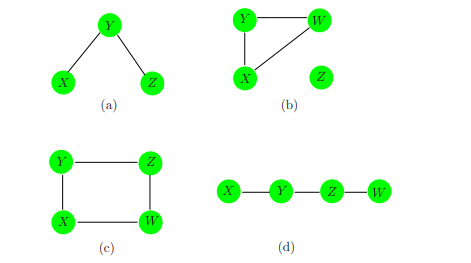
\includegraphics[width=8cm, height=4cm]{Graphs}
\end{frame}
\begin{frame}
\frametitle{Density function}
Probability density function over graph $G$, can be represented as:
\begin{equation}
f(x)=\frac{1}{Z}\prod_{c \in C}{\psi_c(x_c)}
\end{equation}
where $C$ is the set of maximal cliques and $\psi_c$ are clique potentials and \begin{equation}
Z=\sum_{x \in X} f(x)
\end{equation}
\end{frame}
\begin{frame}
\frametitle{Density function}
Probability density function over graph $G$, can be represented as:
\begin{equation}
f(x)=\frac{1}{Z}\prod_{c \in C}{\psi_c(x_c)}
\end{equation}
where $C$ is the set of maximal cliques and $\psi_c$ are clique potentials and 
\begin{equation}
Z=\sum_{x \in X} f(x)
\end{equation}
\end{frame}
\begin{frame}
\frametitle{Dependence structure}
\begin{itemize}
\item Consider three-node clique. It could represent the dependence structure of the distributions:
\begin{equation}
f_2(x,y,z)=\frac{1}{Z}*\psi(x,y)*\psi(x,z)*\psi(y,z)
\end{equation}
\begin{equation}
f_3(x,y,z)=\frac{1}{Z}*\psi(x,y,z)
\end{equation}
\end{itemize}

\includegraphics[width=15cm, height=4cm]{Graph}
\end{frame}
\begin{frame}
\frametitle{Undirected Graphical Models for Continuous Variables}
\begin{itemize}
\item Consider three-node clique. It could represent the dependence structure of the distributions:
\begin{equation}
f_2(x,y,z)=\frac{1}{Z}*\psi(x,y)*\psi(x,z)*\psi(y,z)
\end{equation}
\begin{equation}
f_3(x,y,z)=\frac{1}{Z}*\psi(x,y,z)
\end{equation}
\end{itemize}

\includegraphics[width=15cm, height=4cm]{Graph}
\end{frame}
\begin{frame}
\frametitle{Undirected Graphical Models for Continuous Variables}
\begin{itemize}
\item Markov graphs where all variables are continouos
\item Multivariate Gaussian distribution
\end{itemize}
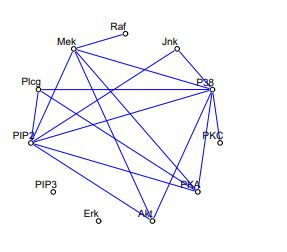
\includegraphics[width=5cm, height=4cm]{Gaussian_image}
\end{frame}
\begin{frame}
\frametitle{Undirected Graphical Models for Continuous Variables}
\end{frame}
\begin{frame}
\frametitle{Gaussian distribution properties}
\begin{itemize}
\item All conditional distributions are also Gaussian
\item The inverse covariance matrix($\theta = \Sigma^{-1}$)
contains information about the partial covariances
\end{itemize}
\end{frame}
\begin{frame}
\frametitle{Example}
\end{frame}
\begin{frame}
\frametitle{Estimation of the Parameters when the Graph Structure is Know}
\begin{itemize}
\item Suppose that we have complete graph (clique)
\item We have N multivariate normal realizations $x_i , i = 1,... ,N$ with population mean $\mu$ and covariance $\Sigma$. Let
\begin{equation}
S=\frac{1}{N}*\sum_{i=1}^{N} (x_i-\overline{x})*(x_i-\overline{x})^T
\end{equation}
where $\overline{x}$ is the sample mean vector.
\item The log-likelihood of data can be written as: 
\begin{equation}
l(\Theta)=log(det(\Theta))-trace(S*\Theta)
\end{equation}
\item $l(\Theta)$ is a convex function of $\Theta$.  Maximum likelihood estimate of $\Sigma$ is simply S 
\end{itemize}
\end{frame}

\begin{frame}
\frametitle{Equality-constrained convex optimization problem}
\begin{itemize}
\item We assume that graphs are not complete(some edges are missing)
\item We would like to maximize
(10) under the constraints that some pre-defined subset of the parameters are zero.
\item A number of methods have been proposed for solving it
\item We outline a simple alternate approach 
\end{itemize}
\end{frame}

\begin{frame}
\frametitle{Alternate approach}
\begin{itemize}
\item Idea is based on linear regression
\item We want to estimate values $\theta_{i,j}$ for given $i$
\item We use model-based estimate of the cross-product matrix of the predictors when we perform our regressions
\end{itemize}
\end{frame}

\begin{frame}
\frametitle{Alternate approach - details}
\begin{itemize}
\item We add Lagrange constants for all missing edges:
\begin{equation}
l_C(\Theta)=log(det(\Theta))-trace(S*\Theta)-\sum_{(j, k)\notin E}{\gamma_{jk}*\theta_{jk}}
\end{equation}
\item Gradient equation for maximizing (11) can be written as:
\begin{equation}
\Theta^{-1} - S - \Gamma = 0
\end{equation}
where $\Gamma$ is a matrix of Lagrange parameters.
\item We will solve for $\Theta$ and its inverse $W = \Theta^{-1}$ one row and column at a time.
\end{itemize}
\end{frame}
\begin{frame}
\frametitle{Alternate approach - details ctd.}
\begin{itemize}
\item For simplicity let’s focus on the
last row and column. Then the upper right block of equation (12) can be written as
\begin{equation}
w_{12}-s_{12}-\gamma_{12}=0
\end{equation}
\item Let's say that matrices $W$ and $\Theta$ are written as:
$\begin{pmatrix}
W_{11} & w_{12}\\
w_{12}^T & w_{22}
\end{pmatrix} * \begin{pmatrix}
\Theta_{11} & \theta_{12}\\
\theta_{12}^T & \theta_{22} 
\end{pmatrix} = \begin{pmatrix}
I & 0\\
0^T & 1 
\end{pmatrix}$ 
\item We can see that:
\begin{equation}
W_{11} * \theta_{12} + w_{12}*\theta_{22}=0 \iff w_{12}=\frac{-W_{11}*\theta_{12}}{\theta_{22}}
\end{equation}
\item Let's say $\beta = −\theta_{12} / \theta_{22}$
\end{itemize}
\end{frame}

\begin{frame}
\frametitle{Alternate approach - details ctd.}
\begin{itemize}

\item Let's say $\beta = −\theta_{12} / \theta_{22}$
\item Then 
\begin{equation}
W_{11}*\beta-s_{12}-\gamma_{12} = 0
\end{equation}
\item These can be interpreted as the $p - 1$ estimating equations for the regression of $X_p$ on the other predictors.
\item To solve (15) we will use subset regression.
\end{itemize}
\end{frame}

\begin{frame}
\frametitle{Subset regression}
\begin{itemize}
\item Suppose there are $p−q$ nonzero elements in $\gamma_{12}$
\item By removing these $p-q$ elements (and also reducing $\beta$ to $\beta^*$ by removing its p − q zero elements. We get system of q equations:
\begin{equation}
W_{11}^* * \beta^* - s_{12}^* = 0
\end{equation}
with solution $\beta^* = (W_{11}^*)^{-1} * s_{12}^*$, which filled with zeros gives us solution $\beta$
\item We can also calculate $\theta_{12}$, because 
\begin{equation}
\frac{1}{\theta_{22}} = w_{22} - w_{12}^T * \beta
\end{equation}
\end{itemize}
\end{frame}
\begin{frame}
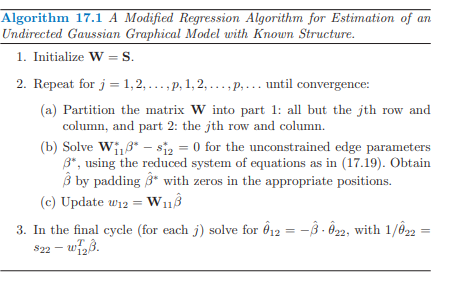
\includegraphics[width=10cm, height=6cm]{Algorithm linear regression}
\end{frame}

\begin{frame}
\frametitle{Estimation of the graph structure}
\begin{itemize}
\item In most cases we do not know which edges to omit from our graph.
\item We would like to discover this from the data itself.
\item We will use Lasso regression.
\end{itemize}
\end{frame}

\begin{frame}
\frametitle{Estimation of the graph structure ctd.}
\begin{itemize}
\item Let's consider maximizing the penalized
log-likelihood:
\begin{equation}
log(det(\Theta))-trace(S*\Theta)-\lambda*||\Theta||_1
\end{equation}
\item We can adapt the lasso to give the exact maximizer of the penalized log-likelihood
\end{itemize}
\end{frame}

\begin{frame}
\frametitle{Estimation of the graph structure ctd.}
\begin{itemize}
\item The analog of the gradient equation:
\begin{equation}
\Theta^{-1} - S - \lambda*Sign(\Theta) = 0
\end{equation}
\item We assume that if $\theta_{jk} = 0$ then $Sign(\theta_{jk}) \in \{-1, 1\}$ and otherwise it is singum function.
\item Next we can have analogue of (15):
\begin{equation}
W_{11}*\beta - s_{12} + \lambda * sign(\beta) = 0
\end{equation}
\item This system is equivalent to the estimating equations for a lasso regression
\end{itemize}
\end{frame}

\begin{frame}
\frametitle{Lasso recall}
\begin{itemize}
\item Recall that with outcome variables y and predictor matrix Z, lasso minimizes
\begin{equation}
\frac{1}{2} * (y - Z * \beta)^T * (y - Z * \beta) + \lambda * ||\beta||_1
\end{equation}
\item Gradient of this expression is:
\begin{equation}
Z^T*Z*\beta - Z^T * y + \lambda * Sign(\beta) = 0
\end{equation}
If we replace $Z^T *y$ with $s_{12}$ and $Z^T * Z$ with $W_{11}$ we have analog of (20)
\end{itemize}
\end{frame}
\begin{frame}
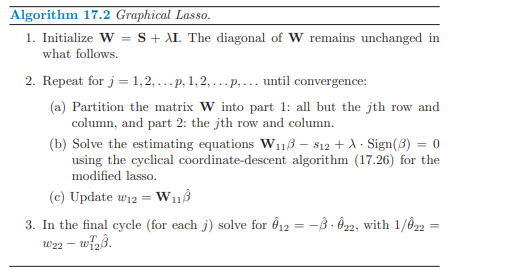
\includegraphics[width=10cm, height=6cm]{Algorithm lasso}
\end{frame}

\begin{frame}
\frametitle{Coordinate descent method}
\begin{itemize}
\item Let $V=W_{11}$. The update has form:
\begin{equation}
\beta_j \leftarrow \frac{S(s_{12j}-\sum_{k \neq j}V_{kj}*\beta_k, \lambda)}{V_{jj}}
\end{equation}
where $S$ is the soft-threshold operator
\begin{equation}
S(x, t)=sign(x) * (|x| - t)_+
\end{equation}
\item The procedure cycles through the predictors until convergence.
\end{itemize}
\end{frame}

\begin{frame}
\frametitle{Grpahical example}
\includegraphics[width=7cm, height=6cm]{lasso solutions}
\end{frame}

\begin{frame}
\frametitle{Undirected Graphical Models for Discrete Variables}
\end{frame}

\begin{frame}
\frametitle{Undirected Graphical Models for Discrete Variables}
\begin{itemize}
\item Markov networks with all variables being discrete
\item The most common are pairwise Markov networks with binary variables
\item Sometimes called Ising models or Boltzmann machines
\end{itemize}
\end{frame}

\begin{frame}
\frametitle{Undirected Graphical Models for Discrete Variables ctd.}
\begin{itemize}
\item Let $X_j$ be binary valued variable at node $j$. The Ising model for their joint  probabilities:
\begin{equation}
P(X, \Theta) = exp\Big[\sum_{j \neq k} \theta_{jk} * X_j * X_k - \Phi(\Theta)\Big]
\end{equation}
where $X \in \{0, 1\}^p$ and $\Phi(\Theta)$ is the log of the partition function
\begin{equation}
\Phi(\Theta)=log \sum_{x \in \{0, 1\}^p} \Big[exp \Big( \sum_{(j, k) \in E} \theta_{jk} * x_j * x_k \Big) \Big] 
\end{equation}
\item The Ising model implies a logistic form for each node conditional on the others. Let's say that $X_{-j}$ means all of the nodes except j.
\begin{equation}
Pr(X_j=1 | X_{-j}=x_{-j})=\frac{1}{1 + exp(-\theta_{j0} - \sum_{(j, k) \in E} \theta_{jk} * x_k)}
\end{equation}
\end{itemize}
\end{frame}

\begin{frame}
\frametitle{ Estimation of the Parameters when the Graph Structure is Known}
\begin{itemize}
\item Suppose we have observations $x_i \in \{0,1\}^p$
\item The log-likelihood is
\begin{equation}
l(\theta) = \sum_{i=1}^N log( P(X_i = x_i, \Theta)) = \sum_{i=1}^N (\sum_{(j, k) \in E} \theta_{jk} * x_{ij} * x_{ik} - \Phi(\Theta))
\end{equation} 
\item Gradient of log-likelihood is:
\begin{equation}
\frac{\partial l(\Theta)}{\partial \theta_{jk}} = \sum_{i=1}^N x_{ij} * x_{ik} - N * \frac{\partial \Phi(\Theta)}{\partial \theta_{jk}} 
\end{equation}
where
\begin{equation}
\frac{\partial \Phi(\Theta)}{\partial \theta_{jk}}  = \sum_{x \in \{0, 1\}^p} x_j * x_k * p(x, \Theta)= E_{\Theta}(X_jX_k)
\end{equation}
\end{itemize}
\end{frame}

\begin{frame}
\frametitle{ Estimation of the Parameters when the Graph Structure is Known ctd.}
\begin{itemize}
\item If we set gradient to zero we will have 
\begin{equation}
E( X_jX_k ) − E_{\Theta}(X_jX_k) = 0
\end{equation}
Where 
\begin{equation}
E( X_jX_k )= \frac{1}{N} * \sum_{i=1}^N x_{ij} * x_{ik} 
\end{equation}
\item If p is not so big, we can use bunch of methods to solve it.
\end{itemize}
\end{frame}

\begin{frame}
\frametitle{ Poisson log-linear modeling}
\begin{itemize}
\item We treat problem as regression problem.
\item Vector y is the vector of $2^p$ counts in each of the possible distribution.
\item Matrix Z has $2^p$ rows and up to $1+p+p^2$ columns that characterize each of the distribution
\item Cost is $O(p^4 * 2^p)$. 
\end{itemize}
\end{frame}

\begin{frame}
\frametitle{ Poisson log-linear modeling}
\begin{itemize}
\item We treat problem as regression problem.
\item Vector y is the vector of $2^p$ counts in each of the possible distribution.
\item Matrix Z has $2^p$ rows and up to $1+p+p^2$ columns that characterize each of the distribution
\item Cost is $O(p^4 * 2^p)$. 
\end{itemize}
\end{frame}

\begin{frame}
\frametitle{ Estimation, when p is big}
\begin{itemize}
\item Let's say $p > 30$. In this case we can approximate the gradient with methods:
   %\subitem Mean field approximation - TODO
\end{itemize}
\end{frame}

\begin{frame}
\frametitle{ Hidden Nodes}
\begin{itemize}
\item We can make Markov's graph complexity better by including hidden nodes.
\item Let $X_H$ be the subset of hidden nodes and reminder $X_V$ be the subset of visible nodes. Then the observed log-likelihood of the observed data is:
\begin{align*}
l(\Theta) = \sum_{i=1}^N log[Pr_{\Theta}(X_V = x_{iV})] = \\ \sum_{i=1}^N log\Big[\sum_{x_H \in \chi_H} exp \sum_{(j, k) \in E} (\theta_{jk} * x_{ij} * x_{ik} - \Phi(\Theta))\Big]
\end{align*}
\end{itemize}
\end{frame}

\begin{frame}
\frametitle{ Hidden Nodes - ctd.}
\begin{itemize}
\item The gradient is:
\begin{equation}
\frac{\partial l(\Theta)}{\partial \theta_{jk}} = E_{V} * E_{\Theta}(X_jX_k|X_v) -  E_{\Theta}(X_jX_k)
\end{equation}
\item The value of the first term depends whether variables $X_j$ and $X_k$ are hidden or not. If both are visible $E_V$ is mean of them. If one or both are hidden, they are first imputed given the visible data, and then averaged over the hidden variables.
\item $E_{\theta}(X_jX_k | X_v)$ is given by formula:
\[E_{\theta}(X_jX_k | X_v = x_{iv}) = \begin{cases}
    x_{ij}*x_{ik}       & \quad \text{if } j, k \in V\\
     x_{ij}*Pr_{\Theta}(X_k = 1 | X_V = x_{iV})       & \quad \text{if } j \in V, k \in H\\
     Pr_{\Theta}(X_j = 1, X_k = 1 | X_V = x_{iV})       & \quad \text{if } j, k \in H\\
\end{cases} 
\]
\end{itemize}
\end{frame}

\begin{frame}
\frametitle{ Estimation of the Graph Structure }
\begin{itemize}
\item{An approximate solution, analogous to the graphical Lasso for continued variables.}
\item{We want to fit an L1-penalized logistic regression model to each node as a function of the other nodes, and then symmetrize the edge parameter estimates in some fashion}
\item{The key difference between estimation of the discrete and continuous models is that in the continuous case, both $\Theta$ and its inverse will often be of interest, while discrete case only yields $\Theta$}
\end{itemize}
\end{frame}

\begin{frame}
\frametitle{ Restricted Boltzmann Machines }
TODO: Think if this slide is neccessary
\end{frame}
\end{document}
%\column{0.5\textwidth}
%    \begin{block}{Right Column}
%      this is a block
%    \end{block}